\documentclass[11pt,a4paper]{article}
\usepackage[utf8]{inputenc}
\usepackage{amsmath}
\usepackage{mathtools}
\usepackage{amsfonts}
\usepackage{amssymb}
\usepackage{graphicx}
\usepackage{caption}
\usepackage{subcaption}
\usepackage{comment}
\usepackage{color}
\usepackage{enumitem}
\usepackage[left=2cm,right=2cm,top=2cm,bottom=2cm]{geometry}
\usepackage{listings}
\usepackage{color}

\setlength{\jot}{10pt}
 
\definecolor{codegreen}{rgb}{0,0.6,0}
\definecolor{codegray}{rgb}{0.5,0.5,0.5}
\definecolor{codepurple}{rgb}{0.58,0,0.82}
\definecolor{backcolour}{rgb}{0.95,0.95,0.92}
 
\lstdefinestyle{mystyle}{
    backgroundcolor=\color{backcolour},   
    commentstyle=\color{codegreen},
    keywordstyle=\color{magenta},
    numberstyle=\tiny\color{codegray},
    stringstyle=\color{codepurple},
    basicstyle=\footnotesize,
    breakatwhitespace=false,         
    breaklines=true,                 
    captionpos=b,                    
    keepspaces=true,                 
    numbers=left,                    
    numbersep=5pt,                  
    showspaces=false,                
    showstringspaces=false,
    showtabs=false,                  
    tabsize=2
}
 
\lstset{style=mystyle}
\author{Andrew Teta}
\title{ECEN 4532 - Lab 3: Perspective Transformations and Motion Tracking}
\date{February 25, 2019}

\begin{document}

\maketitle

\begin{figure}[ht]
	\centering
	\begin{subfigure}[h]{0.6\textwidth}
		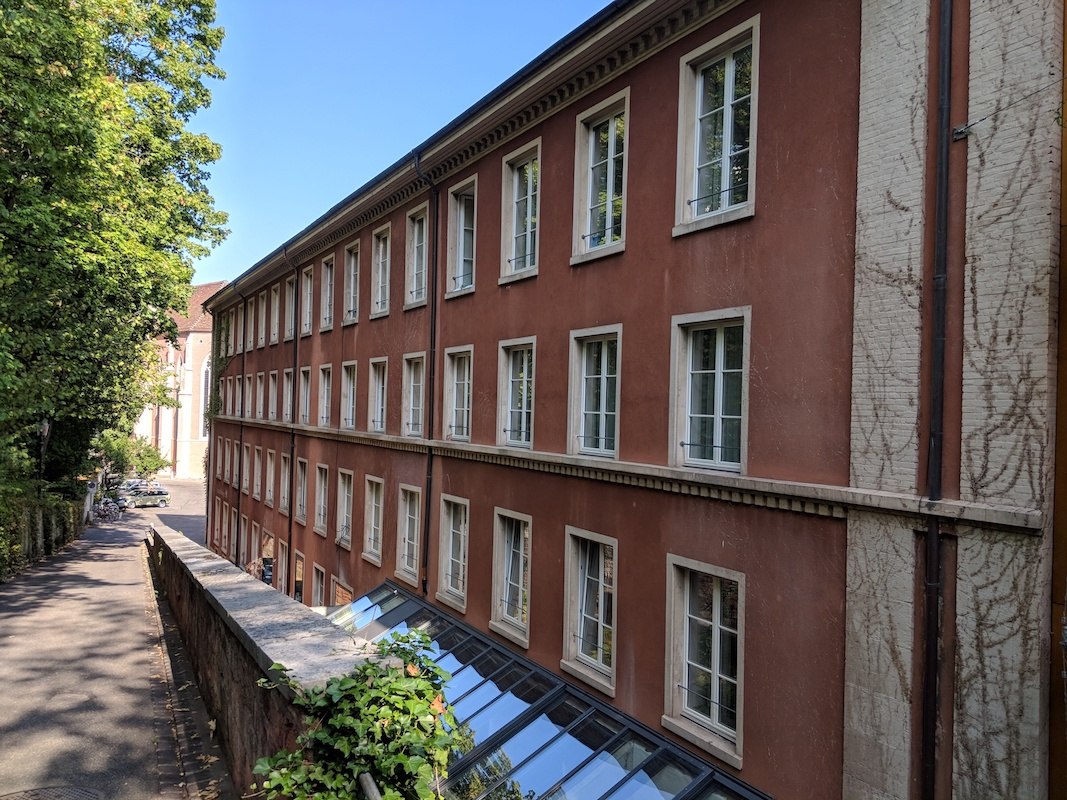
\includegraphics[width=\textwidth]{PC_test_2}
	\end{subfigure}
	\par\bigskip
	\begin{subfigure}[h]{0.6\textwidth}
		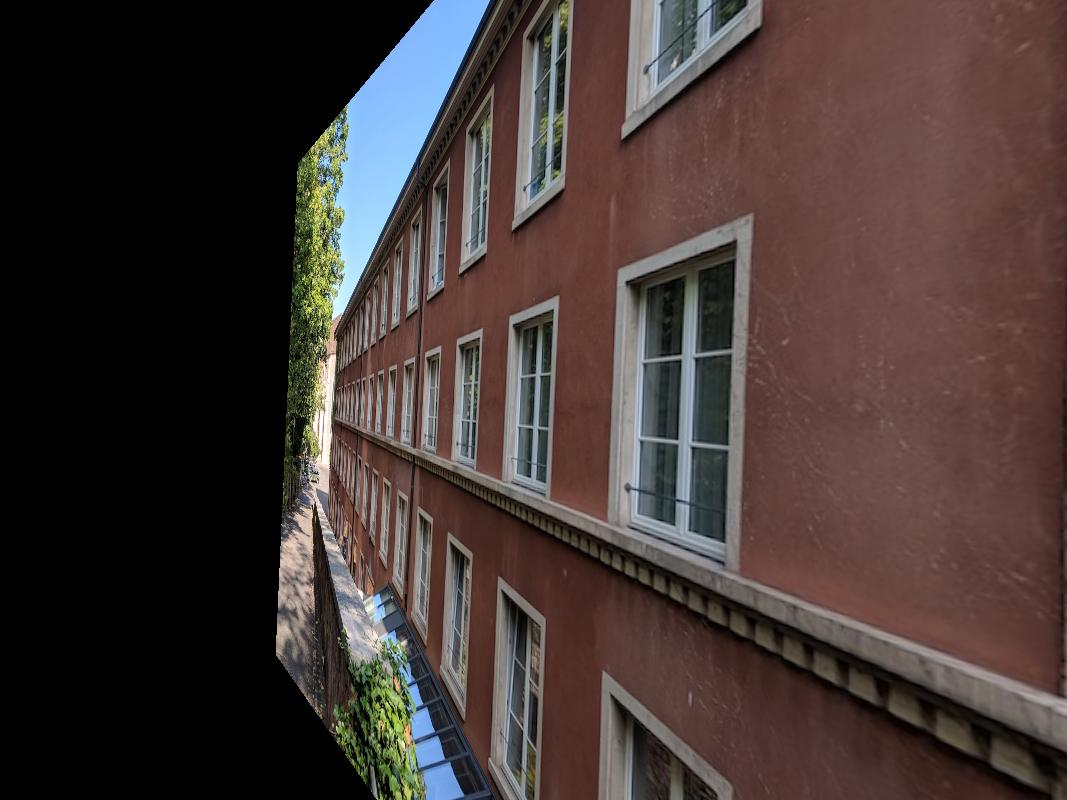
\includegraphics[width=\textwidth]{out1}
	\end{subfigure}
\end{figure}

\pagebreak

\tableofcontents

\pagebreak

\addcontentsline{toc}{section}{Introduction}
\section{Introduction}
In this lab, we explore the low-level implementation of perspective distortion correction, and a simplified model of video motion tracking between frames in Python. We will mostly use \verb|numpy| to manipulate N-D arrays of pixel information. Additionally, I used a free photo editing software called GIMP to select pixel indexes.

\subsection{Background}
Our algorithm for perspective distortion correction relies on the math theory of linear algebra, using a linear transformation matrix to map pixels from one image to another. Then, the process of motion tracking between frames will be based on a series of image pyramids, using block-based motion estimation to "search" for a matching region in the next frame.

\section{Perspective Distortion Correction}
\subsection{Linear Regression}
We begin by defining linear regression as one approach to modeling the relationship between a dependent and independent variable. This method is commonly used to fit a model to an \textbf{over-determined} set of data points. By over-determined, we mean there are more equations defining the data set, than there are variables, often occurring when many measurements are performed to estimate a small number of parameters. 

Mathematically, we have a relationship of the form, $Ax=c$, where A is over-determined. This only has a solution if \textbf{c} lies in the column space of A, however there will not be an exact solution if A is over-determined and we instead seek an \textbf{x} that minimizes the mean-squared-error (MSE), defined $E=|A\textbf{x}-\textbf{b}|^2$. Ultimately, we want to find a "pseudo-inverse", $A^+$, such that $\textbf{x}^\$=A^+\textbf{c}$

\end{document}